\documentclass[10pt]{beamer}

% === Base packages ===
\usetheme{polimi}
% Usage instructions can be found at: https://github.com/elauksap/beamerthemepolimi
\usecolortheme{default}

\usepackage[utf8]{inputenc}
\usepackage[T1]{fontenc}
\usepackage[english]{babel}
\usepackage{microtype}

% === Math packages ===
\usepackage{amsmath, amssymb, amsfonts, bm, mathtools}
\usepackage{listings}

% === Pictures and figures ===
\usepackage{graphicx}
\usepackage{caption}
\usepackage{tikz} 
\usetikzlibrary{bayesnet, positioning, shapes, arrows.meta}

% === Title ===
\title{Bayesian Constrained-based Structure Learning}
\subtitle{\vspace{-1.5em}Implementation of a new algorithm to perform Bayesian structure\\
learning, mimicking PC algorithm (Sprites et al., 2000)}
\author{Group 9}
\institute{Politecnico di Milano}
\date{November 28, 2025}

% === Bibliography ===
\usepackage[
  backend=biber,
  style=authoryear, % o numeric, apa, ieee, ecc.
  sorting=nyt
]{biblatex}
\addbibresource{references.bib}





\begin{document}
% --- Title ---
\begin{frame}
    \maketitle
\end{frame}

% --- Sections and frame ---
\section{Introduction}
\begin{frame}{\textbf{Motivation}}
  \begin{itemize}
    \item What is structure learning?
    \item Why Bayesian?
    \item Applications in causal inference
  \end{itemize}
\end{frame}

\begin{frame}{\textbf{Graphical Models}}
    \centering
  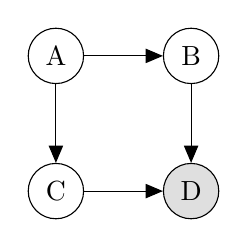
\begin{tikzpicture}
    \node[latent] (A) {A};
    \node[latent, right=of A] (B) {B};
    \node[latent, below=of A] (C) {C};
    \node[obs, right=of C] (D) {D};

    \edge {A} {B, C};
    \edge {B,C} {D};
  \end{tikzpicture}
\end{frame}

\section{Frequentist Approach}
\begin{frame}{\textbf{PC Algorithm}}
    
\end{frame}

\section{Bayesian Approach}
\begin{frame}{\textbf{Prior estimation}}
  \begin{equation}
    p(G, \theta | D) \propto p(D | G, \theta) \, p(\theta | G) \, p(G)
  \end{equation}
\end{frame}

\begin{frame}{\textbf{Bayes factor}}
    
\end{frame}

\section{Next Steps}
\begin{frame}{\textbf{Dataset: Riboflavin Production}}
    %\textbf{Description:} \\
    Dataset of riboflavin production by \textit{Bacillus subtilis} containing 
    $n=71$ observations of $p=4088$ predictors (gene expressions) and a one-dimensional response (riboflavin production).
    
    \medskip
    %\textbf{Usage:} \\
    \texttt{data(riboflavin)}, available in the \texttt{R} package \texttt{hdi}.
    
    \medskip
    %\textbf{Format:} 
    \begin{itemize}
        \item \textbf{y:} Log-transformed riboflavin production rate (original name: \texttt{q\_RIBFLV})
        \item \textbf{x:} (Co-)variables measuring the logarithm of the expression level of 4088 genes
    \end{itemize}
\end{frame}

\section{}
\begin{frame}[allowframebreaks]{\textbf{References}}
    \nocite{*}
    \printbibliography
\end{frame}

\end{document}
